\documentclass{beamer}
\usetheme{Darmstadt}
\useinnertheme{rectangles}
\definecolor{garnet}{RGB}{114,47,55}
\definecolor{darkgarnet}{RGB}{80,30,37}
\definecolor{darkdarkgarnet}{RGB}{57,23,27}
\definecolor{darkdarkdarkgarnet}{RGB}{40,15,18}
\definecolor{gold}{RGB}{212,175,55}
\definecolor{darkgold}{RGB}{150,115,45}
\setbeamercolor{palette primary}{bg=garnet}
\setbeamercolor{palette secondary}{bg=darkgarnet} 
\setbeamercolor{palette tertiary}{bg=darkdarkgarnet}
\setbeamercolor{palette quaternary}{bg=darkdarkdarkgarnet}
\setbeamercolor{background canvas}{bg=white}
\setbeamercolor*{item}{fg=darkgold}
\setbeamercolor{block title}{bg=darkgold}


\title[TAB v2] % (optional, only for long titles)
{The Tagless Access Buffer (TAB)}
\subtitle{An Updated Approach to Reduce Cache Energy Usage with Minimal ISA Changes}
\author{Carlos Sanchez}
\institute[FSU]
{Computer Science Department\\ Florida State University}
\date{Fall 2015}
\subject{Computer Science}

\begin{document} 
\frame{\titlepage} 
\section{Introduction}
\subsection{TAB Basics}
\begin{frame}{What is the Tagless Access Buffer?}
   \begin{itemize}
      \item A small buffer placed at the top of the memory hierarchy
      \item Holds a few lines from the L1D (inclusive)
      \item Data explicitly directed from the L1D to the TAB by compiler 
         generated instructions
      \item Compiler looks in loops for references with constant strides
         or invariant addresses to direct to the TAB
   \end{itemize}
   \begin{center}
      \includegraphics[width=0.8\textwidth]{figures/dmemhier.pdf}
   \end{center}
\end{frame}
\begin{frame}{What problem does it solve?}
   \begin{itemize}
      \item Energy efficiency is a major design constraint in processors
      \item Cache accounts for up to 25\% of a processor's total power draw
      \item TAB reduces overall cache energy usage because it:
         \begin{itemize}
            \item Is smaller than the L1D
            \item Requires far fewer DTLB accesses
            \item Requires no tag check
            \item Is compiler controlled, meaning more analysis on the most
               efficient usage of the structure
         \end{itemize}
   \end{itemize}
\end{frame}
\begin{frame}{Why constant strides or invariant addresses?}
   \begin{itemize}
      \item Can calculate the following reference's address if the loop reference
         has a known constant stride throughout the loop or if the address 
         doesn't change
      \item Knowing this, we can prefetch the next line before it is needed so
         it is available before the next access
      \item No need to check tags; prefetching guarantees the TAB to have the line 
         we need
   \end{itemize}
\end{frame}
\subsection{Operation Introduction}
\begin{frame}{TAB Instructions}
   Two instructions control the TAB. Both instructions use the same opcode,
   distinguished by a bit
   \begin{itemize}
      \item \textbf{gtab} links a register to a TAB entry
      \item once active, references with that base register will be directed to the TAB
      \item gtab prefetches the line needed by the first TAB reference
      \item Further prefetches are performed automatically when needed and keep
         the line data valid for future TAB references
      \item \textbf{rtabs} removes the register link and deallocates the TAB
   \end{itemize}
\end{frame}
\begin{frame}{Example TAB Instruction Generation}
   \begin{center}
      \begin{block}{Original Loop (simple summation)}
         \includegraphics[scale=0.20]{figures/compiler_example_1-1.pdf}
      \end{block}
      \begin{block}{Basic Generated Instructions}
         \includegraphics[scale=0.20]{figures/compiler_example_1-2.pdf}
      \end{block}
      \begin{block}{Compiler Inserted TAB Instructions}
         \includegraphics[scale=0.20]{figures/compiler_example_1-3.pdf}
      \end{block}
   \end{center}
\end{frame}
\section{Hardware}
\subsection{TAB Structures}
\begin{frame}{Required Structures}
   %TAB requires a number of structures for operation:
   \begin{itemize}
      \item The TAB itself to hold a number of lines from the L1D 
         (four in our implementation)
      \item Metadata structure for TAB entry and TAB line metadata
      \item Register array to store the base register associated with
         each TAB (four register numbers)
      \item Valid window structure to indicate TAB validity per function call
         (eight windows, four valid bits per window)
   \end{itemize}
\end{frame}
\begin{frame}{Structure Overview}
   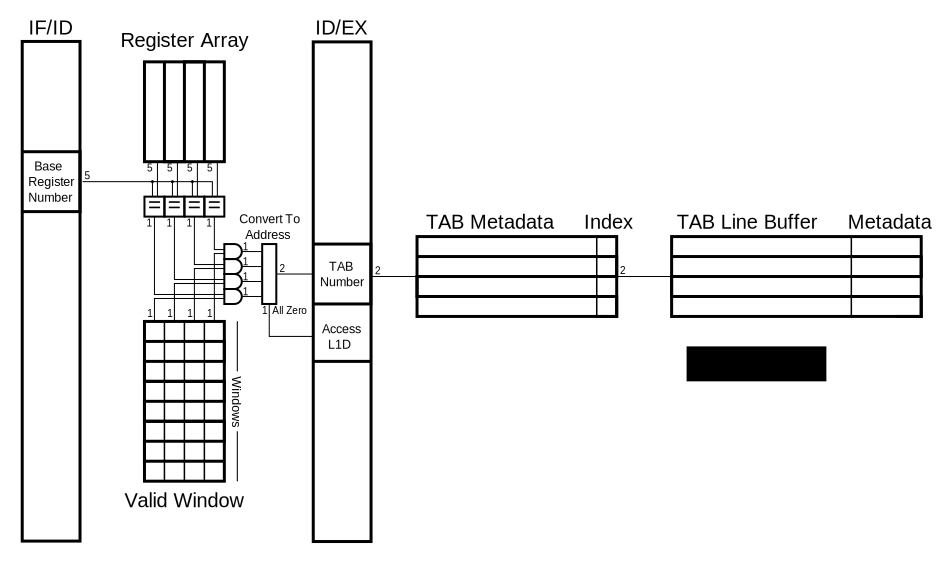
\includegraphics[width=\textwidth]{figures/tabhardware.pdf}
\end{frame}
\begin{frame}{TAB ID Stage}
   \begin{columns} %[c] for centered, [T] for top
      \column{.57\textwidth}
      \begin{block}{TAB Reference Detection}
         \begin{itemize}
            \item Compare memory reference's base register number against
               each TAB associated register number in parallel
            \item If any match AND the matching TAB is valid (\texttt{AND} bits 
               from comparison with current valid window), direct reference to TAB
            \item If none match, go the the L1D
         \end{itemize}
      \end{block}
      \column{.43\textwidth}
      \includegraphics[width=\textwidth]{figures/tabhardware_ID.pdf}
   \end{columns}
\end{frame}
\begin{frame}{How it works with explanation 2}
   \begin{columns} %[c] for centered, [T] for top
      \column{.5\textwidth}
         This is how it works: yeah
      \begin{block}{This is a block}
         A detailed explanation with a fancy header
      \end{block}
      \column{.5\textwidth}
      \begin{block}{An image in a block}
         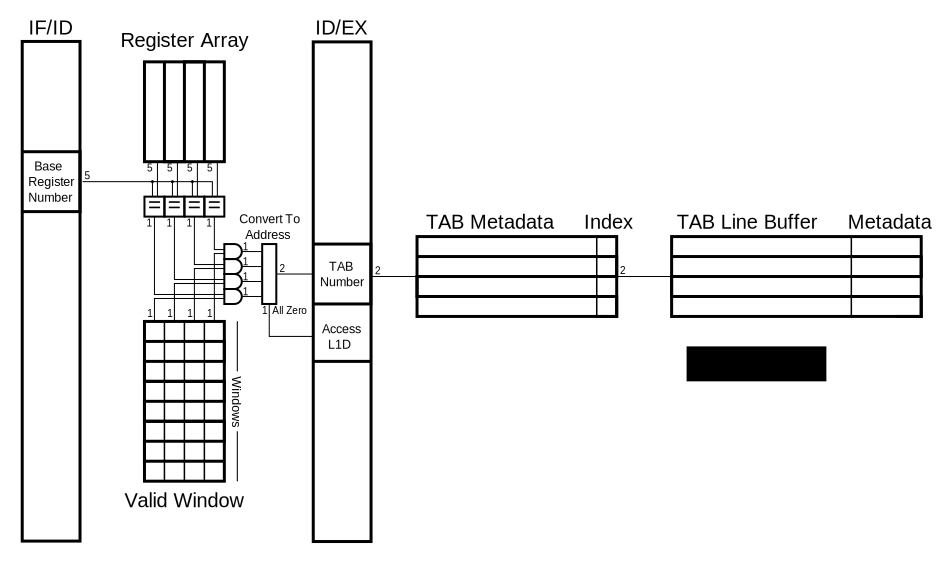
\includegraphics[width=\textwidth]{figures/tabhardware.pdf}
      \end{block}
   \end{columns}
\end{frame}
\end{document}
